%% Robot PU Product Brochure — 2-page, letter paper, front+back
%% Compile: pdflatex robotpu-brochure.tex  (run twice for references)
\documentclass[10pt]{article}

% ── Page geometry ──────────────────────────────────────────────────────────────
\usepackage[
  letterpaper,
  margin=0.5in,
  top=0.45in,
  bottom=0.45in
]{geometry}

% ── Packages ───────────────────────────────────────────────────────────────────
\usepackage[T1]{fontenc}
\usepackage{lmodern}
\usepackage{microtype}
\usepackage{xcolor}
\usepackage{graphicx}
\usepackage{tikz}
\usepackage{multicol}
\usepackage{enumitem}
\usepackage{fontawesome5}        % icons  (install texlive-fonts-extra)
\usepackage{mdframed}
\usepackage{array}
\usepackage{tabularx}
\usepackage{booktabs}
\usepackage{parskip}
\usepackage{url}
\usepackage{qrcode}              % QR code  (install texlive-extra-utils)
\usepackage{tcolorbox}
\tcbuselibrary{skins,breakable}
\usepackage{wrapfig}
\usepackage{setspace}
\usepackage{amssymb}

% ── Colours ────────────────────────────────────────────────────────────────────
\definecolor{puBlue}{HTML}{1565C0}
\definecolor{puCyan}{HTML}{00B0FF}
\definecolor{puOrange}{HTML}{FF6D00}
\definecolor{puGray}{HTML}{455A64}
\definecolor{puLight}{HTML}{E3F2FD}
\definecolor{puDark}{HTML}{0D47A1}
\definecolor{puGreen}{HTML}{2E7D32}
\definecolor{puYellow}{HTML}{F9A825}
\definecolor{pageBg}{HTML}{F0F7FF}

% ── No page numbers ────────────────────────────────────────────────────────────
\pagestyle{empty}

% ── Helpers ────────────────────────────────────────────────────────────────────
\newcommand{\featurebox}[3]{%
  \begin{tcolorbox}[
      colback=#1!8,
      colframe=#1,
      arc=3pt,
      boxrule=1pt,
      left=3pt, right=3pt, top=2pt, bottom=2pt,
      fonttitle=\bfseries\footnotesize\color{white},
      title={\textcolor{white}{#2}},
      coltitle=white,
      attach boxed title to top left={xshift=5pt,yshift=-2pt},
      boxed title style={colback=#1,arc=2pt}
    ]
    \footnotesize #3
  \end{tcolorbox}
}

\newcommand{\tutrow}[3]{%
  \textcolor{#1}{\textbf{#2}} & \small #3 \\[1pt]
}

% ── Document ───────────────────────────────────────────────────────────────────
\begin{document}

% ════════════════════════════════════════════════════════════════════════════════
%  PAGE 1 — Product Overview
% ════════════════════════════════════════════════════════════════════════════════
\pagecolor{pageBg}

% ── Header bar ─────────────────────────────────────────────────────────────────
\begin{tikzpicture}[remember picture, overlay]
  \fill[puDark] (current page.north west) rectangle
    ([yshift=-1.5cm]current page.north east);
  \node[anchor=west, xshift=0.55in, yshift=-0.75cm,
        text=white, font=\bfseries\Large] at (current page.north west)
    {Robot\,PU \quad\textcolor{puCyan}{|}\quad
     \textit{\normalsize The Playful, Programmable micro:bit Robot}};
  \node[anchor=east, xshift=-0.55in, yshift=-0.75cm,
        text=white, font=\bfseries\small] at (current page.north east)
    {\textcolor{puYellow}{\faGlobe}\; robotgyms.com/pu};
\end{tikzpicture}

\vspace{1.4cm}

% ── Two-column layout: image left, quick-facts right ───────────────────────────
\begin{minipage}[t]{0.48\linewidth}
  \vspace{0pt}
  \begin{center}
    \includegraphics[width=\linewidth,height=5.8cm,keepaspectratio]%
      {../product/robotpu.png}
  \end{center}
  \vspace{2pt}
  \begin{center}
    \includegraphics[width=0.55\linewidth,height=2.2cm,keepaspectratio]%
      {../product/robotpu_gamepad.png}\\[2pt]
    {\footnotesize\color{puGray} Robot PU with gamepad remote control}
  \end{center}
\end{minipage}%
\hfill
\begin{minipage}[t]{0.49\linewidth}
  \vspace{0pt}

  % tagline
  {\large\bfseries\color{puDark}
   Walk. Dance. Talk. Navigate. Code.}

  \vspace{4pt}
  {\footnotesize\color{puGray}
  A complete, classroom-ready robot built on the \textbf{BBC micro:bit V2}.
  From elementary classrooms to college robotics labs, Robot PU turns
  abstract STEM concepts into hands-on, creative projects.
  Add the optional \textbf{ESP32-S3 Smart Hat} to unlock AI-camera
  perception, soccer, and SLAM navigation.}

  \vspace{6pt}

  % What's in the kit
  \featurebox{puBlue}{\faBox\; What's in the Kit}{%
    \begin{itemize}[leftmargin=12pt, itemsep=0pt, topsep=0pt]
      \item Robot PU body (pre-built \& upgradable)
      \item 2 $\times$ micro:bit compatible boards
      \item Gamepad for radio remote control
      \item Printed manual \& quick-start guide
      \item Access to 60+ online tutorials, games \& projects
    \end{itemize}
  }

  \vspace{4pt}

  % Coding paths
  \featurebox{puGreen}{\faCode\; Three Coding Paths}{%
    \begin{tabularx}{\linewidth}{@{}lX@{}}
      \textbf{Blocks} & Drag-and-drop MakeCode blocks \\
      \textbf{JS/TS}  & Typed JavaScript / TypeScript \\
      \textbf{Python} & Python package (NovaSeq/RobotPu) \\
    \end{tabularx}
  }

  \vspace{4pt}

  % Optional add-on
  \featurebox{puOrange}{\faMicrochip\; Optional: ESP32-S3 Smart Hat}{%
    Adds AI camera, voice commands, SLAM navigation, face detection,
    object tracking, and robot soccer autonomy. \textit{Sold separately.}
  }
\end{minipage}

\vspace{6pt}
\noindent\textcolor{puCyan}{\rule{\linewidth}{1.5pt}}
\vspace{4pt}

% ── Features row ───────────────────────────────────────────────────────────────
\begin{multicols}{4}

  % col 1
  \begin{center}
    
\includegraphics[height=1.2cm,keepaspectratio]{../cartoons/pu_dance.png}
  \end{center}
  {\small\bfseries\color{puDark}Walk \& Express}\\
  {\footnotesize
    Walk, turn, side-step, kick, jump, rest.
    Dance routines that react to music beats.
    Talk \& sing with RoboVoice. Blinking LED eyes show mood.}

  \columnbreak

  % col 2
  \begin{center}
    
\includegraphics[height=1.2cm,keepaspectratio]{../cartoons/pu_walk.png}
  \end{center}
  {\small\bfseries\color{puDark}Autopilot \& Navigation}\\
  {\footnotesize
    Sonar obstacle avoidance. Maze solving.
    Path following. Local planner. Leader following.
    Decision engine for guided missions.}

  \columnbreak

  % col 3
  \begin{center}
    
\includegraphics[height=1.2cm,keepaspectratio]{../cartoons/pu_ideas.png}
  \end{center}
  {\small\bfseries\color{puDark}Sensing \& Control}\\
  {\footnotesize
    Sonar, IMU tilt/roll/pitch, compass heading, microphone input.
    Signal filtering, heading fusion, and PID balance control.
    Servo trim calibration \& kinematics.}

  \columnbreak

  % col 4
  \begin{center}
    
\includegraphics[height=1.2cm,keepaspectratio]{../cartoons/pu_star.png}
  \end{center}
  {\small\bfseries\color{puDark}Multi-Robot \& AI}\\
  {\footnotesize
    Radio gamepad, peer-to-peer chat, synchronized singing.
    Formation control, task allocation, ROS-inspired architecture.
    AI camera soccer \& SLAM (Smart Hat).}

\end{multicols}

\vspace{3pt}
\noindent\textcolor{puCyan}{\rule{\linewidth}{1pt}}
\vspace{2pt}

% ── Bottom bar: purchase / links + cartoon decoration ──────────────────────────
\begin{minipage}[c]{0.72\linewidth}
  \begin{tabular}{@{}ll@{}}
    \textcolor{puBlue}{\faShoppingCart} &
      \textbf{Amazon:} \url{amazon.com/dp/B0DR8RGVXN} \\[3pt]
    \textcolor{puBlue}{\faGlobe} &
      \textbf{Website:} \url{robotgyms.com/pu} \\[3pt]
    \textcolor{puBlue}{\faYoutube} &
      \textbf{YouTube:} The Story of PU (\url{youtube.com/@TheStoryofPu-yw8tr}) \\[3pt]
    \textcolor{puBlue}{\faGithub} &
      \textbf{Open Source:} \url{github.com/robotgyms/pxt-robotpu} \\[3pt]
    \textcolor{puBlue}{\faMicrochip} &
      \textbf{MakeCode:} \url{makecode.microbit.org} — add extension \texttt{robotgyms/pxt-robotpu} \\
  \end{tabular}
\end{minipage}%
\hfill
\begin{minipage}[c]{0.25\linewidth}
  \begin{center}
    
\includegraphics[height=2.2cm,keepaspectratio]{../cartoons/pu_happy.png}\\
    {\footnotesize\color{puGray}\textit{Meet PU!}}
  \end{center}
\end{minipage}

% ════════════════════════════════════════════════════════════════════════════════
%  PAGE 2 — Tutorial Contents
% ════════════════════════════════════════════════════════════════════════════════
\newpage
\pagecolor{pageBg}

% ── Header bar ─────────────────────────────────────────────────────────────────
\begin{tikzpicture}[remember picture, overlay]
  \fill[puDark] (current page.north west) rectangle
    ([yshift=-1.5cm]current page.north east);
  \node[anchor=west, xshift=0.55in, yshift=-0.75cm,
        text=white, font=\bfseries\Large] at (current page.north west)
    {Robot\,PU \quad\textcolor{puCyan}{|}\quad
     \textit{\normalsize 60+ Tutorials — From First Code to Real Robotics}};
  \node[anchor=east, xshift=-0.55in, yshift=-0.75cm,
        text=white, font=\bfseries\small] at (current page.north east)
    {\textcolor{puYellow}{\faGlobe}\; robotgyms.com/pu};
\end{tikzpicture}

\vspace{1.4cm}

% ── Age-band intro ─────────────────────────────────────────────────────────────
\begin{tcolorbox}[
    colback=puDark,
    colframe=puDark,
    arc=6pt,
    left=8pt, right=8pt, top=5pt, bottom=5pt
  ]
  \centering
  \textcolor{white}{\bfseries\small
    {\color{puYellow}\faGraduationCap}\;
    Ages 8--10 \textbf{Beginner} \quad
    \textcolor{puCyan}{$\bullet$} \quad
    Ages 11--13 \textbf{Intermediate} \quad
    \textcolor{puCyan}{$\bullet$} \quad
    Ages 14--17 \textbf{Advanced} \quad
    \textcolor{puCyan}{$\bullet$} \quad
    Difficulty:
    {\color{puYellow}$\bigstar$} Beginner\;
    {\color{puYellow}$\bigstar\bigstar$} Intermediate\;
    {\color{puYellow}$\bigstar\bigstar\bigstar$} Advanced}
\end{tcolorbox}

\vspace{4pt}

% ── 3-column tutorial grid ─────────────────────────────────────────────────────
\begin{multicols}{3}

% ---- Column 1 ----------------------------------------------------------------
\featurebox{puBlue}{\faRocket\; Setup \& Basics}{%
  {\footnotesize
  \begin{tabular}{@{}p{0.06\linewidth}p{0.78\linewidth}@{}}
    {\color{puYellow}$\bigstar$}   & Project skeleton \\
    {\color{puYellow}$\bigstar$}   & Hello world demo \\
    {\color{puYellow}$\bigstar\bigstar$} & JavaScript / TypeScript quick start \\
  \end{tabular}}
}

\vspace{3pt}

\featurebox{puBlue}{\faWrench\; Build \& Calibration}{%
  {\footnotesize
  \begin{tabular}{@{}p{0.06\linewidth}p{0.78\linewidth}@{}}
    {\color{puYellow}$\bigstar$}   & Add arms \\
    {\color{puYellow}$\bigstar$}   & Servo trim calibration \\
  \end{tabular}}
}

\vspace{3pt}

\featurebox{puBlue}{\faRunning\; Robot Hardware \& APIs}{%
  {\footnotesize
  \begin{tabular}{@{}p{0.06\linewidth}p{0.78\linewidth}@{}}
    {\color{puYellow}$\bigstar$}   & How Robot PU moves \\
    {\color{puYellow}$\bigstar$}   & Robot actions \\
    {\color{puYellow}$\bigstar\bigstar$} & Robot observation \\
    {\color{puYellow}$\bigstar\bigstar$} & Don't bonk \\
  \end{tabular}}
}

\vspace{3pt}

\featurebox{puGreen}{\faMusic\; Music, Speech \& Expression}{%
  {\footnotesize
  \begin{tabular}{@{}p{0.06\linewidth}p{0.78\linewidth}@{}}
    {\color{puYellow}$\bigstar$}   & Music + beat-driven behaviors \\
    {\color{puYellow}$\bigstar$}   & Dance choreography \\
    {\color{puYellow}$\bigstar\bigstar$} & Music library utilities \\
    {\color{puYellow}$\bigstar\bigstar$} & Emotion state to expression \\
    {\color{puYellow}$\bigstar\bigstar$} & RoboVoice melodic speech \\
    {\color{puYellow}$\bigstar\bigstar$} & Talk content patterns \\
    {\color{puYellow}$\bigstar\bigstar$} & Synchronized singing \\
  \end{tabular}}
}

\vspace{3pt}

\featurebox{puGreen}{\faGamepad\; Fun Projects}{%
  {\footnotesize
  \begin{tabular}{@{}p{0.06\linewidth}p{0.78\linewidth}@{}}
    {\color{puYellow}$\bigstar\bigstar$} & Kungfu pose sequence \\
    {\color{puYellow}$\bigstar\bigstar\bigstar$} & Learn to skate \\
  \end{tabular}}
}

\columnbreak

% ---- Column 2 ----------------------------------------------------------------
\featurebox{puOrange}{\faWifi\; Communication \& Control}{%
  {\footnotesize
  \begin{tabular}{@{}p{0.06\linewidth}p{0.78\linewidth}@{}}
    {\color{puYellow}$\bigstar$}   & Remote control \\
    {\color{puYellow}$\bigstar$}   & Gamepad patterns \\
    {\color{puYellow}$\bigstar\bigstar$} & Peer chat over radio \\
  \end{tabular}}
}

\vspace{3pt}

\featurebox{puOrange}{\faCodeBranch\; Programming Structure}{%
  {\footnotesize
  \begin{tabular}{@{}p{0.06\linewidth}p{0.78\linewidth}@{}}
    {\color{puYellow}$\bigstar\bigstar$} & Event loop \\
    {\color{puYellow}$\bigstar\bigstar$} & Custom events \& handlers \\
    {\color{puYellow}$\bigstar\bigstar$} & State machines \\
    {\color{puYellow}$\bigstar\bigstar$} & OOP architecture \\
  \end{tabular}}
}

\vspace{3pt}

\featurebox{puOrange}{\faMap\; Navigation \& Mapping}{%
  {\footnotesize
  \begin{tabular}{@{}p{0.06\linewidth}p{0.78\linewidth}@{}}
    {\color{puYellow}$\bigstar\bigstar$} & Sonar operator \\
    {\color{puYellow}$\bigstar\bigstar$} & Maze solving \\
    {\color{puYellow}$\bigstar\bigstar$} & Autopilot navigation \\
    {\color{puYellow}$\bigstar\bigstar$} & 2D mapping concepts \\
    {\color{puYellow}$\bigstar\bigstar\bigstar$} & Submarine sonar project \\
    {\color{puYellow}$\bigstar\bigstar\bigstar$} & Leader-following decision engine \\
    {\color{puYellow}$\bigstar\bigstar\bigstar$} & Occupancy grid \\
    {\color{puYellow}$\bigstar\bigstar\bigstar$} & Shared mapping \\
    {\color{puYellow}$\bigstar\bigstar\bigstar$} & Path planning \\
    {\color{puYellow}$\bigstar\bigstar\bigstar$} & Path following \\
    {\color{puYellow}$\bigstar\bigstar\bigstar$} & Local planner \\
  \end{tabular}}
}

\vspace{3pt}

\begin{center}
  
\includegraphics[height=1.8cm,keepaspectratio]{../cartoons/pu_questions.png}
  
\includegraphics[height=1.8cm,keepaspectratio]{../cartoons/pu_jump.png}
\end{center}

\columnbreak

% ---- Column 3 ----------------------------------------------------------------
\featurebox{puGray}{\faSitemap\; ROS Concepts}{%
  {\footnotesize
  \begin{tabular}{@{}p{0.06\linewidth}p{0.78\linewidth}@{}}
    {\color{puYellow}$\bigstar\bigstar$} & ROS nodes as roles \\
    {\color{puYellow}$\bigstar\bigstar$} & ROS topics on micro:bit \\
    {\color{puYellow}$\bigstar\bigstar$} & /cmd\_vel topic \\
    {\color{puYellow}$\bigstar\bigstar$} & /scan topic \\
    {\color{puYellow}$\bigstar\bigstar$} & /diagnostics topic \\
    {\color{puYellow}$\bigstar\bigstar\bigstar$} & Telemetry logging \\
    {\color{puYellow}$\bigstar\bigstar\bigstar$} & Base station dashboard \\
    {\color{puYellow}$\bigstar\bigstar\bigstar$} & Safety watchdog + E-stop \\
    {\color{puYellow}$\bigstar\bigstar\bigstar$} & Fault recovery behaviors \\
    {\color{puYellow}$\bigstar\bigstar\bigstar$} & Behavior trees \\
    {\color{puYellow}$\bigstar\bigstar\bigstar$} & Mission recipes \\
    {\color{puYellow}$\bigstar\bigstar\bigstar$} & Task allocation \\
    {\color{puYellow}$\bigstar\bigstar\bigstar$} & Formation control \\
  \end{tabular}}
}

\vspace{3pt}

\featurebox{puGray}{\faCalculator\; Control \& Math}{%
  {\footnotesize
  \begin{tabular}{@{}p{0.06\linewidth}p{0.78\linewidth}@{}}
    {\color{puYellow}$\bigstar\bigstar\bigstar$} & Transformation matrix \\
    {\color{puYellow}$\bigstar\bigstar\bigstar$} & Feedback loops \\
    {\color{puYellow}$\bigstar\bigstar\bigstar$} & Signal filters \\
    {\color{puYellow}$\bigstar\bigstar\bigstar$} & Heading fusion \\
    {\color{puYellow}$\bigstar\bigstar\bigstar$} & PID balancing \\
    {\color{puYellow}$\bigstar\bigstar\bigstar$} & Improved balancing \\
  \end{tabular}}
}

\vspace{3pt}

\featurebox{puOrange}{\faCamera\; Vision, AI \& Soccer SLAM}{%
  {\footnotesize
  \begin{tabular}{@{}p{0.06\linewidth}p{0.78\linewidth}@{}}
    {\color{puYellow}$\bigstar\bigstar\bigstar$} & K230 AI camera \\
    {\color{puYellow}$\bigstar\bigstar\bigstar$} & Search \& track face \\
    {\color{puYellow}$\bigstar\bigstar\bigstar$} & SLAM I2C camera message \\
    {\color{puYellow}$\bigstar\bigstar\bigstar$} & SLAM odometry \\
    {\color{puYellow}$\bigstar\bigstar\bigstar$} & SLAM soccer ball follow \\
    {\color{puYellow}$\bigstar\bigstar\bigstar$} & SLAM soccer local map \\
  \end{tabular}}
}

\end{multicols}

\vspace{2pt}
\noindent\textcolor{puCyan}{\rule{\linewidth}{1pt}}
\vspace{2pt}

% ── Bottom bar ─────────────────────────────────────────────────────────────────
\begin{minipage}[c]{0.32\linewidth}
  \begin{center}
    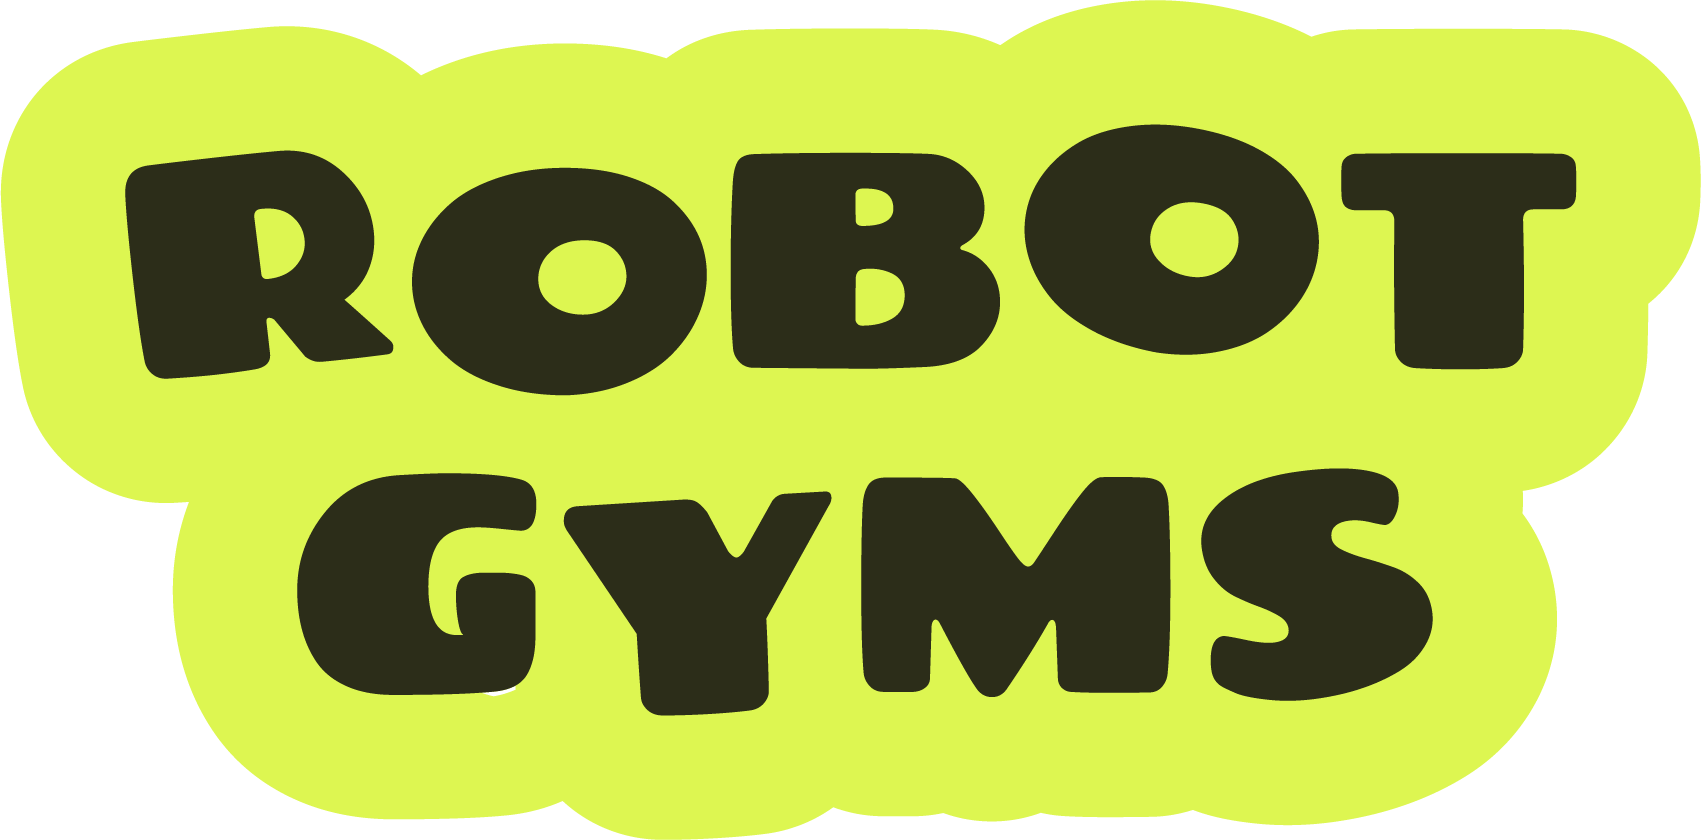
\includegraphics[height=1.6cm,keepaspectratio]{../brand/robotgyms_logo.png}
  \end{center}
\end{minipage}%
\hfill
\begin{minipage}[c]{0.35\linewidth}
  \centering
  {\small\bfseries\color{puDark}The Story of PU — Learning Books}\\[3pt]
  {\footnotesize
  \textcolor{puBlue}{Book 1} Pair Up \;|\;
  \textcolor{puBlue}{Book 2} Games \;|\;
  \textcolor{puBlue}{Book 3} Growth\\
  \textcolor{puBlue}{Book 4} Journey \;|\;
  \textcolor{puBlue}{Book 5} AI Camera\\[3pt]
  \url{robotgyms.com/pu}}
\end{minipage}%
\hfill
\begin{minipage}[c]{0.28\linewidth}
  \begin{center}
    
\includegraphics[height=1.6cm,keepaspectratio]{../cartoons/pu_sing.png}
    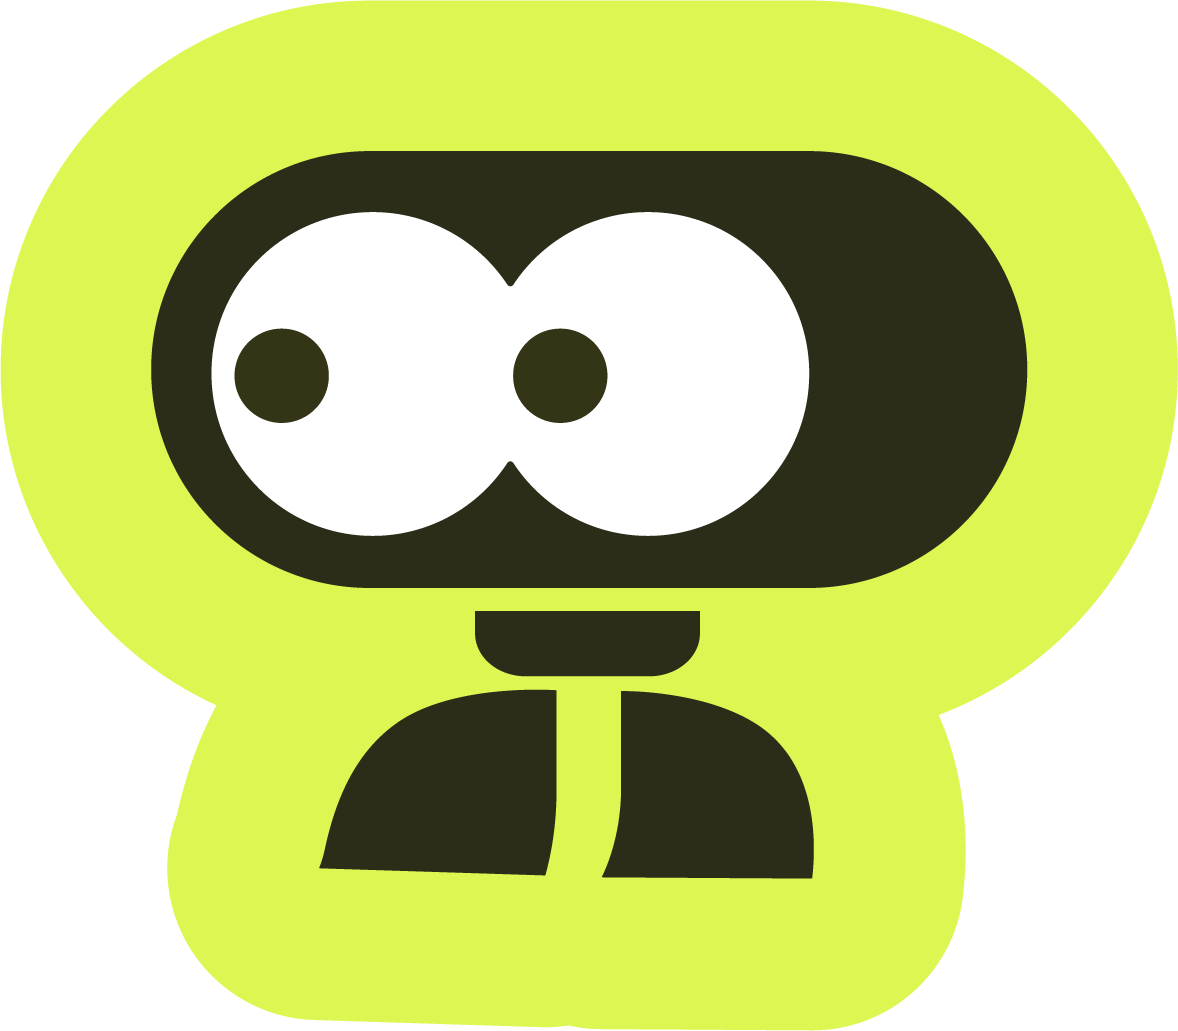
\includegraphics[height=1.6cm,keepaspectratio]{../cartoons/pu_supprise.png}
  \end{center}
\end{minipage}

\end{document}
